%
% einleitung.tex -- Beispiel-File für die Einleitung
%
% (c) 2020 Prof Dr Andreas Müller, Hochschule Rapperswil
%
% !TEX root = ../../buch.tex
% !TEX encoding = UTF-8
%
\section{Die $\Gamma$-Funktion als Erweiterung der Fakultät\label{gamma:section:teil0}}
\kopfrechts{Fakultät erweitern}

Die Erweiterung der Fakultät beschäftigt grosse Namen der Mathematik schon lange.
Eine erste Definition der Fakultät für nicht natürliche Zahlen wird bereits 1720 von Daniel Bernoulli und Christian Goldbach gegeben.
\index{Goldbach, Christian}%
\index{Bernoulli, Daniel}%
Auch Leonhard Euler und James Stirling steuern im Laufe der Jahrhunderte ihre eigene Definition bei. 
\index{Euler, Leonhard}%
\index{Stirling, James}%

\subsection{Bohr-Mollerup-Theorem}\label{gamma:section:BMT}

Um eine Funktion zu finden, welche die Fakultät erweitert, wird das Bohr-Mollerup-Theorem \cite{mollerup1922laerebog} verwendet. Es werden folgende Eigenschaften definiert:
\index{Bohr, Harald}%
\index{Mollerup, Johannes}%
\index{Satz!von Bohr-Mollerup}%

\begin{enumerate}
\item\label{gamma-eq:bm-1}$f(1) = 1$,
\item\label{gamma-eq:bm-2}$f(x+1) = x \cdot f(x), x > 0$,
\item\label{gamma-eq:bm-3}$f(x) \text{ ist logarithmisch konvex}$.
\end{enumerate}

\noindent
Eine Funktion, welche die Eigenschaften~\ref{gamma-eq:bm-1},~\ref{gamma-eq:bm-2} und~\ref{gamma-eq:bm-3} erfüllt,
kann als Erweiterung der Fakultät für nicht natürliche Zahlen betrachtet werden.

Die Eigenschaft~\ref{gamma-eq:bm-1} ist selbsterklärend.
Die Eigenschaft~\ref{gamma-eq:bm-2} verlangt, dass die Funktion rekursiv definiert werden kann.
Die Fakultät erfüllt das, da $5! = 5 \cdot 4!$ ist.
Die Eigenschaft~\ref{gamma-eq:bm-3} verlangt logarithmische Konvexität, was informell als ``wächst schnell'' verstanden werden kann.
Die formelle Definition folgt im nächsten Abschnitt.

\subsubsection{Logarithmische Konvexität}

Eine Kurve ist konvex, wenn diese wie $f(x) = x^2+1$ nach oben geöffnet ist.
Von \emph{logarithmischer Konvexität} spricht man wenn, nach der Anwendung des Logarithmus, die resultierende Funktion auch konvex ist. 
\index{logarithmisch konvex}%
Die Funktion $f(x) = x^2+1$ ist zum Beispiel nicht logarithmisch konvex, denn die zweite Ableitung des Logarithmus ist stellenweise negativ, wie die Abb. \ref{gamma-fig:nonLogConvex} aufzeigt.

\begin{figure}
  \centering
  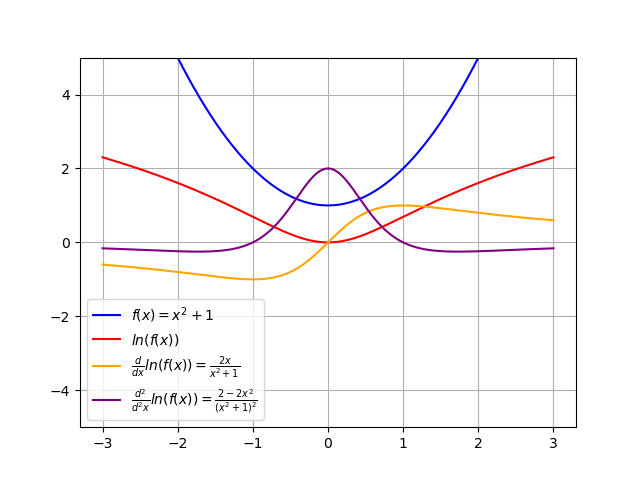
\includegraphics[width=0.8\textwidth]{papers/gamma/img/log_nonconvex.png}
  \caption{Visualisierung der nicht erfüllten logarithmischen Konvexität von $f(x) = x^2+1$.}
\label{gamma-fig:nonLogConvex}
\end{figure}

Ein Beispiel einer logarithmisch konvexen Funktion ist
\begin{equation}
  \label{gamma-eq:logConvex}
  g(x) = e^{x^2} \quad \Rightarrow \quad \log(g(x)) = \log\left(e^{x^2}\right) = x^2,
\end{equation}
deren logarithmische Konvexität auch in Abb. \ref{gamma-fig:logConvex} dargestellt wird.

\begin{figure}
  \centering
  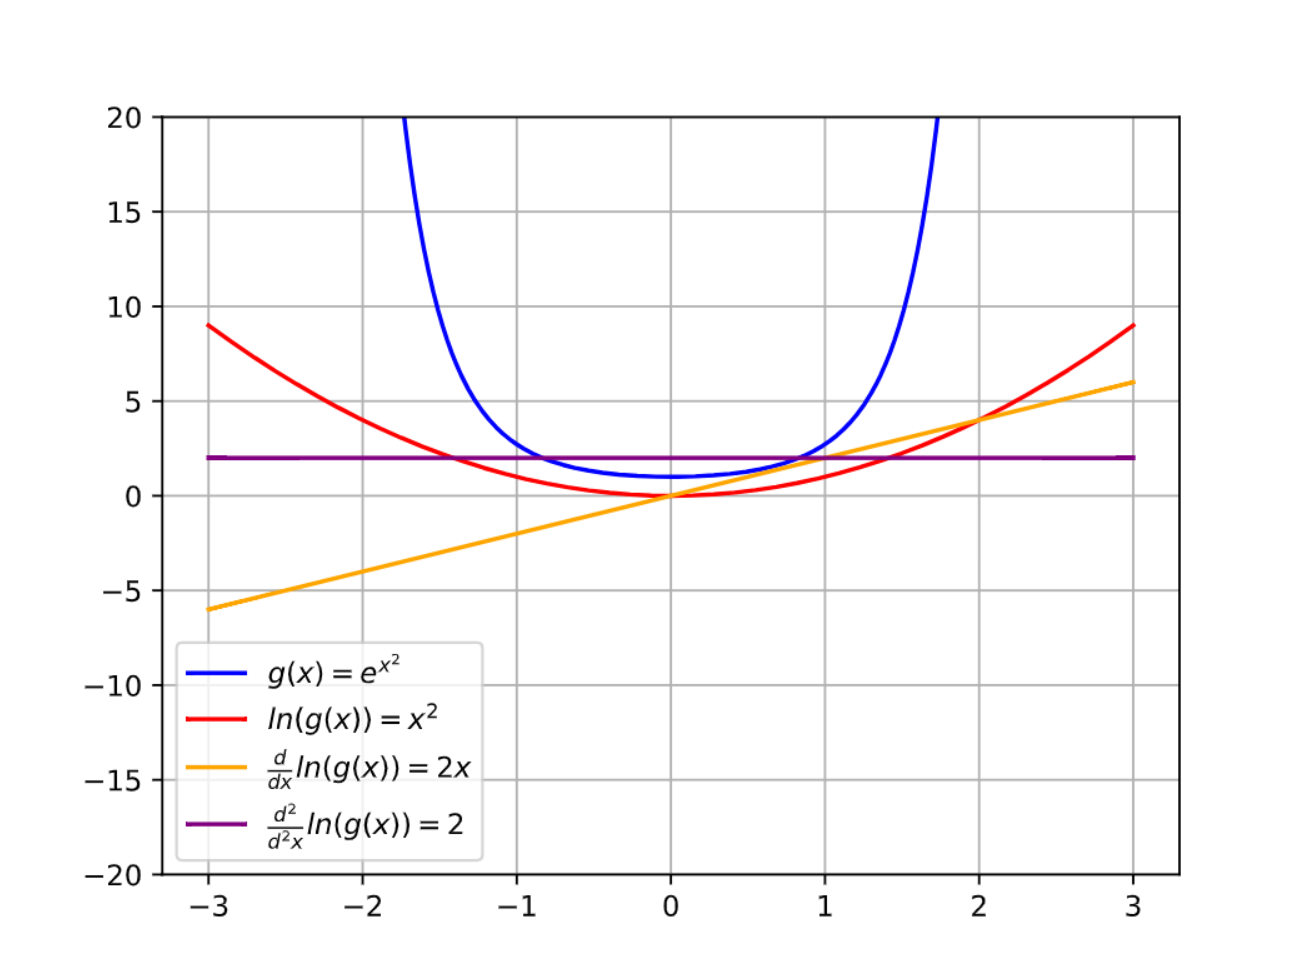
\includegraphics[width=0.8\textwidth]{papers/gamma/img/log_convex_3.png}
  \caption{Visualisierung der logarithmischen Konvexität von $g(x) = e^{x^2}$.}
\label{gamma-fig:logConvex}
\end{figure}

\subsubsection{Suche nach einer passenden Funktion}

Eine Funktion, welche Eigenschaften \ref{gamma-eq:bm-1} und \ref{gamma-eq:bm-2} erfüllt, lässt sich verhältnismässig leicht finden.
Als Beispiel, nimmt man die Funktion
\begin{equation}
\label{gamma-eq:sinusFunction}
    f : \interval[open left, soft open fences]{0}{1} \to \mathbb{R} \quad x \mapsto 2\sin(2 \pi x)+1,
\end{equation}
wird Eigenschaft~\ref{gamma-eq:bm-1} durch die Verschiebung nach rechts bereits erfüllt. Sie kann dann gemäss Eigenschaft~\ref{gamma-eq:bm-2} rekursiv auf
\begin{equation}
\label{gamma-eq:rec-sinus-function}
    \tilde{f} : \mathbb{R} \to \mathbb{R} \quad x \mapsto \begin{cases}
        x^{-1} \cdot f(x+1) & x \leq 0 \\
        2\sin(2 \pi x)+1   & 0 < x \leq 1 \\
        x \cdot f(x-1)     & x > 1
\end{cases}
\end{equation}
erweitert werden und erfüllt somit diese auch.

Wie die Grafik~\ref{gamma-fig:almostGammaFunction} zeigt, nimmt~\eqref{gamma-eq:rec-sinus-function} die bekannten Fakultätswerte an.
Die Ausschläge nach unten und oben zeigen grafisch, dass die logarithmische Konvexität (Eigenschaft~\ref{gamma-eq:bm-3}) für diese Funktion nicht gegeben sein kann.

\begin{figure}
  \centering
  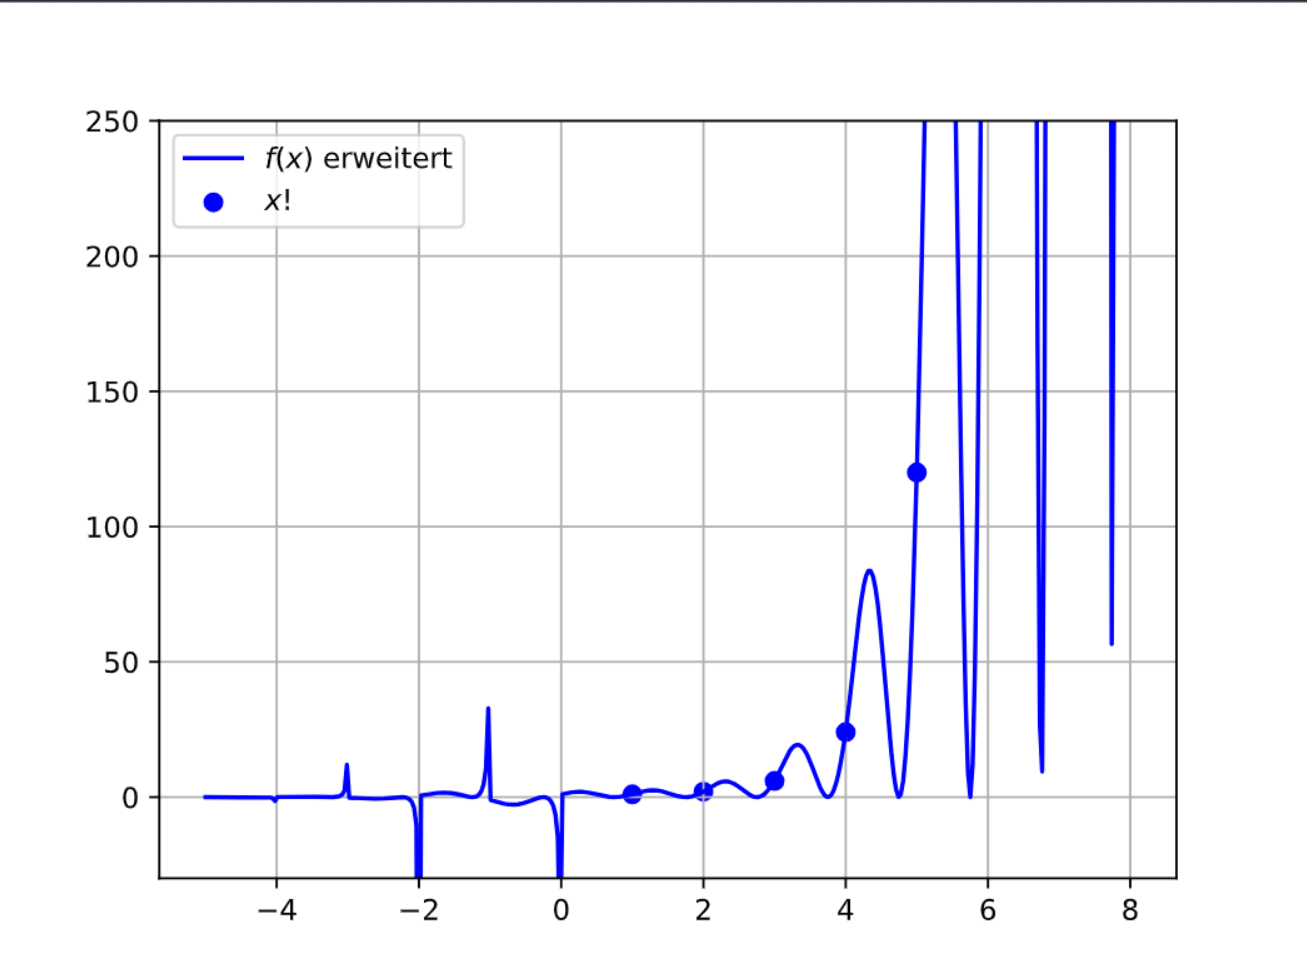
\includegraphics[width=0.8\textwidth]{papers/gamma/img/sin_extended.png}
  \caption{Funktion $f(x)$, welche zwei (\ref{gamma-eq:bm-1} und~\ref{gamma-eq:bm-2}) von drei Eigenschaften des Bohr-Mollerup-Theorems erfüllt.}
\label{gamma-fig:almostGammaFunction}
\end{figure}

Gesucht wird eine Funktion, welche alle Eigenschaften, welche als Teil des Bohr-Mollerup-Theorems definiert wurden, erfüllt.
Die Herleitung der $\Gamma$-Funktion ist nicht trivial und wird deshalb weggelassen (Beispiele in \ref{gamma:section:formulas}).
\index{Gamma@$\Gamma$}%
Interessant ist die Hauptaussage des Bohr-Mollerup-Theorems: die $\Gamma$-Funktion erfüllt als einzige Funktion alle Eigenschaften und ist somit die eindeutige Erweiterung der Fakultät \cite{mollerup1922laerebog}.
